\chapter{M\'odulo de Pacientes}

\section{Descripci\'on General}

El m\'odulo de pacientes gestiona las mascotas registradas en el sistema,
vinculadas a sus due\~nos (clientes). Cada paciente tiene informaci\'on
detallada incluyendo especie, raza, g\'enero, historial de peso y datos
m\'edicos.

\section{Server Actions}

El archivo \texttt{lib/actions/patients.ts} implementa 5 server actions.

\subsection{getPatients --- Listado con Join}

\begin{lstlisting}[style=typescript, caption=getPatients - Listado con join a clientes]
export async function getPatients() {
  const clinicId = await getCurrentClinicId();
  return db
    .select({
      id: schema.patients.id,
      name: schema.patients.name,
      species: schema.patients.species,
      breed: schema.patients.breed,
      gender: schema.patients.gender,
      birthDate: schema.patients.birthDate,
      active: schema.patients.active,
      createdAt: schema.patients.createdAt,
      clientId: schema.patients.clientId,
      clientName: schema.clients.name,
    })
    .from(schema.patients)
    .innerJoin(schema.clients,
      eq(schema.patients.clientId, schema.clients.id))
    .where(eq(schema.patients.clinicId, clinicId))
    .orderBy(desc(schema.patients.createdAt));
}
\end{lstlisting}

\subsection{getPatient --- Detalle Completo}

\begin{lstlisting}[style=typescript, caption=getPatient - Seleccion explicita de columnas]
export async function getPatient(id: number) {
  const row = await db
    .select({
      id: schema.patients.id,
      clientId: schema.patients.clientId,
      name: schema.patients.name,
      species: schema.patients.species,
      breed: schema.patients.breed,
      gender: schema.patients.gender,
      birthDate: schema.patients.birthDate,
      color: schema.patients.color,
      weight: schema.patients.weight,
      microchip: schema.patients.microchip,
      photoUrl: schema.patients.photoUrl,
      allergies: schema.patients.allergies,
      notes: schema.patients.notes,
      active: schema.patients.active,
      createdAt: schema.patients.createdAt,
      updatedAt: schema.patients.updatedAt,
      clientName: schema.clients.name,
      clientPhone: schema.clients.phone,
      clientEmail: schema.clients.email,
    })
    .from(schema.patients)
    .innerJoin(schema.clients,
      eq(schema.patients.clientId, schema.clients.id))
    .where(eq(schema.patients.id, id))
    .then((rows) => rows[0] ?? null);

  return row;
}
\end{lstlisting}

\section{P\'aginas}

\subsection{Listado (/patients)}

\begin{itemize}[leftmargin=*]
    \item Vista en formato tarjetas (\texttt{Card}) con grid responsivo.
    \item Cada tarjeta muestra: nombre, especie (con icono), raza, sexo,
          due\~no y edad calculada.
    \item Enlaces a detalle y edici\'on.
\end{itemize}

\subsection{Creaci\'on (/patients/new)}

\begin{itemize}[leftmargin=*]
    \item Selector de due\~no que carga desde \texttt{GET /api/clients/list}.
    \item Campos: nombre, especie (select con etiquetas en espa\~nol),
          raza, sexo, fecha de nacimiento, color, microchip, alergias, notas.
    \item Validaci\'on b\'asica (sin Zod, usando interfaz TypeScript).
\end{itemize}

\subsection{Detalle (/patients/[id])}

\begin{itemize}[leftmargin=*]
    \item Informaci\'on general: especie, raza, sexo, edad, color, microchip.
    \item Datos del due\~no: nombre, tel\'efono, email.
    \item Alergias y notas destacadas.
    \item Bot\'on ``Historial Cl\'{\i}nico'' que enlaza a
          \texttt{/medical-records?patientId=X}.
    \item Historial de pesos (JSONB renderizado).
\end{itemize}

\section{Componentes}

\begin{itemize}[leftmargin=*]
    \item \textbf{PatientForm:} Componente cliente reutilizable con selector
          de due\~nos que se carga din\'amicamente via fetch.
    \item Los campos de especie y sexo usan \texttt{<select>} nativos con
          etiquetas en espa\~nol desde \texttt{@vetrinaria/shared/constants}.
\end{itemize}

\section{Espec\'{\i}fica de Datos}

El peso se almacena como array JSONB para mantener historial:

\begin{lstlisting}[style=typescript, caption=Campo weight como JSONB]
weight: jsonb('weight')
  .$type<{ value: number; date: string }[]>()
  .default([])
\end{lstlisting}

Esto permite registrar m\'ultiples mediciones de peso con su fecha
correspondiente, habilitando gr\'aficos de evoluci\'on ponderal.

\begin{figure}[H]
    \centering
    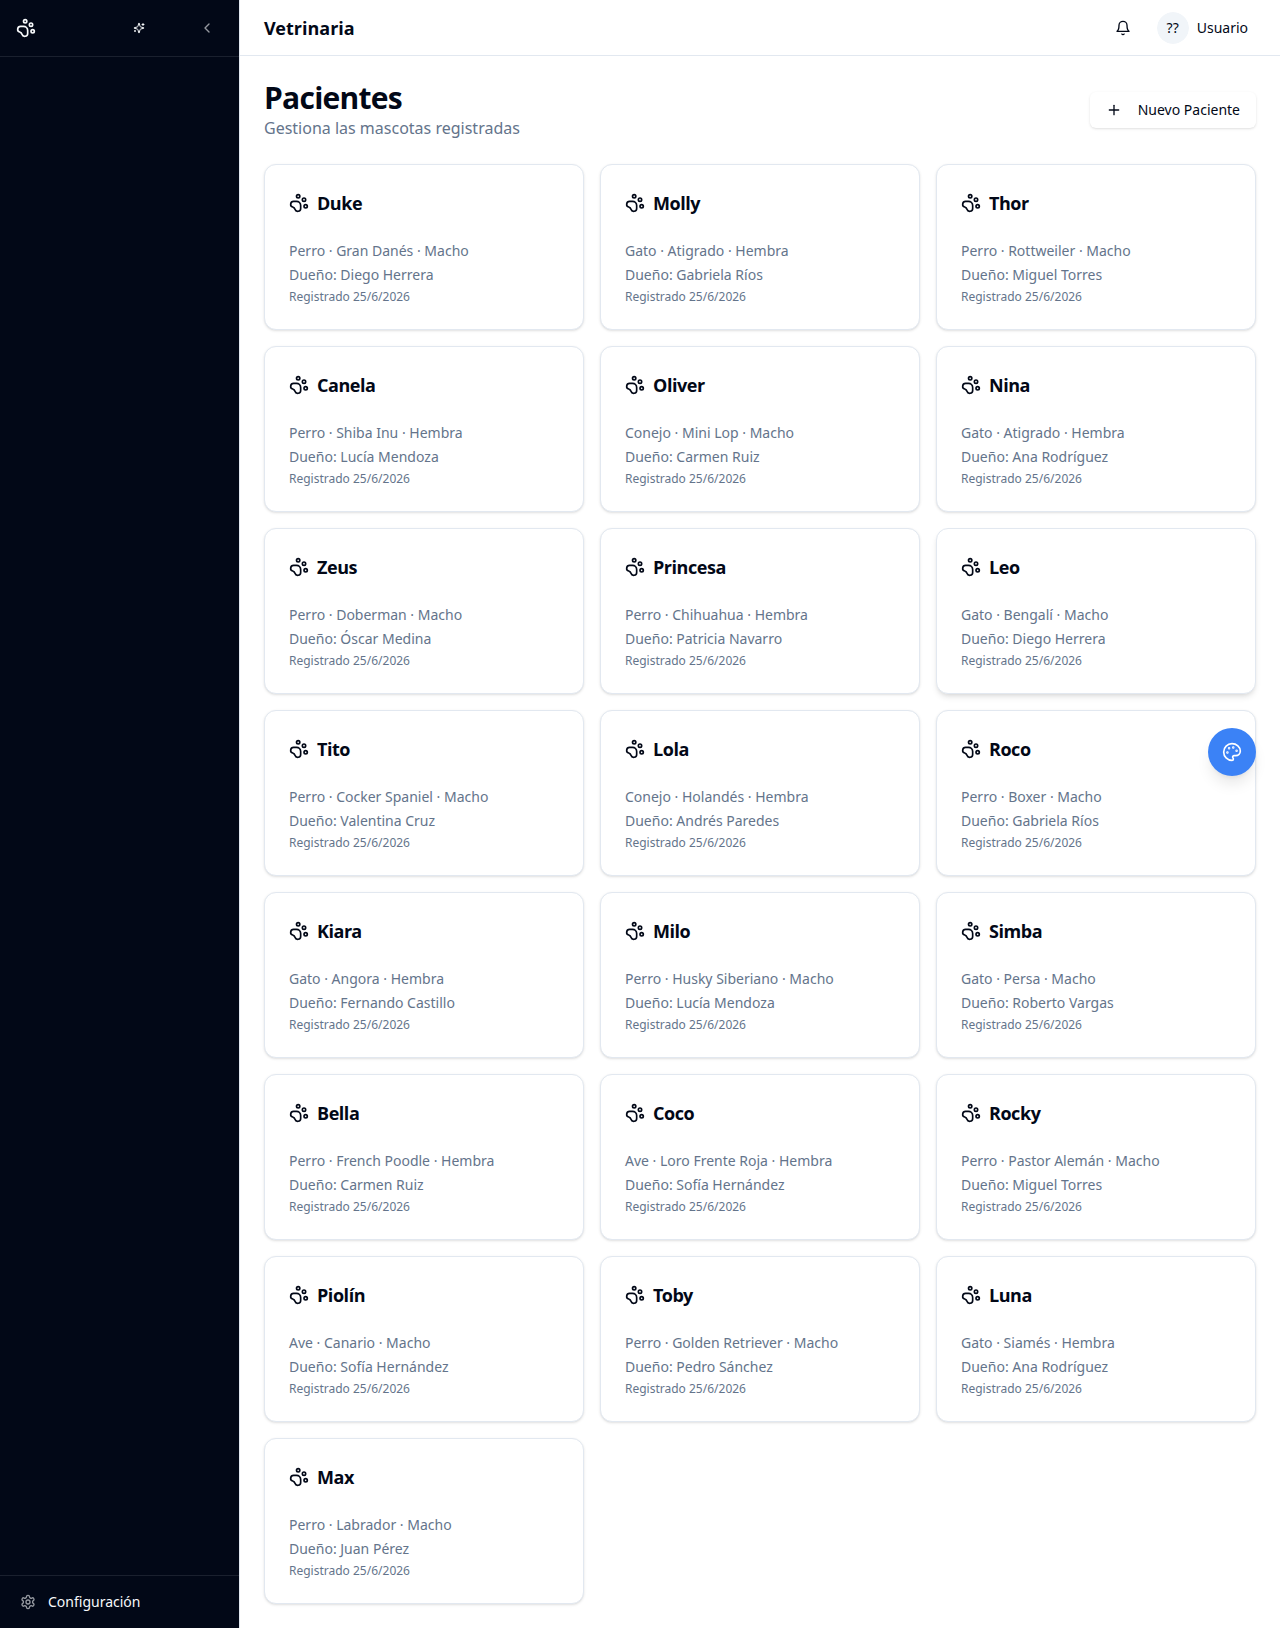
\includegraphics[width=\textwidth]{img/vet-patients.png}
    \caption{Vista de tarjetas de pacientes con informacion de especie y dueno}
    \label{fig:pacientes}
\end{figure}
